\section{Problem Formulation}\label{sec:problem}

\subsection{Conditional causal usefulness}\label{sec:conditional-usefulness}

Let $f$ be a transformer evaluated by a scalar task metric $m$. We consider two executions of the same task instance: an \emph{intact} state $A$ and a \emph{perturbed} state $B$, obtained by applying a prespecified intervention to a primary circuit component or set of components. Let $h$ denote a candidate attention head whose change in functional importance we want to explain. The task metric can differ across applications---for example, an IO-minus-subject logit difference in IOI or the target-token log probability in induction---but it is fixed within an analysis.

For context $s\in\{A,B\}$, let $m_s^{h}$ be the task metric with the candidate head operating normally and let $m_s^{0}$ be the metric when that candidate is zeroed while all other aspects of context $s$ are held fixed. We define the candidate's output-grounded causal usefulness in context $s$ as
\begin{equation}
E_s(h) = m_s^{h}-m_s^{0}.
\label{eq:context-effect}
\end{equation}
The intact and conditional effects are therefore $E_A(h)$ and $E_B(h)$, respectively. The cross-state change we seek to explain is
\begin{equation}
\Delta_h = E_B(h)-E_A(h).
\label{eq:conditional-gain}
\end{equation}
In our experiments this quantity is called \emph{conditional gain}. Positive $\Delta_h$ means that the candidate's contribution becomes more positive after the primary intervention; it does not by itself imply that the candidate is supportive in the perturbed state. We reserve \emph{positive functional recruitment} for cases in which both $E_B(h)>0$ and $\Delta_h>0$. FALI itself is not restricted to positive recruitment: it decomposes positive or negative changes in causal usefulness.

This definition deliberately evaluates the candidate against a zero-candidate baseline in the \emph{same} surrounding context. Consequently, a difference between $E_A(h)$ and $E_B(h)$ cannot be produced merely by a shift in the task metric that affects both the candidate-present and candidate-zero conditions equally. The estimand is the change in the candidate's marginal causal contribution under the specified intervention, not the raw performance difference between states $A$ and $B$.

\subsection{Mechanism-resolution objective}\label{sec:mechanism-objective}

The problem begins after a candidate head and a task-relevant attention target have been chosen. They may come from prior circuit analysis, conditional co-ablation, patching, or a task-specific hypothesis. FALI does not search over heads, discover a target edge, or infer a circuit automatically. Its input is a selected head $h$, two model states $A$ and $B$, a scalar task metric $m$, and a target query--key edge (or prespecified target edge set) whose score is meaningful for the task.

The objective is to account for $\Delta_h$ using changes in three architecture-level objects associated with the candidate: its pre-softmax attention scores, its value vectors, and the surrounding computation in which the resulting head output is used. The score tensor is then resolved more finely into the task-target score, rivals in the same query row, and scores at other query positions. This yields a controlled mechanism-discrimination question: under a fixed intervention algebra, which candidate-local or surrounding changes receive credit for the observed change in output-grounded usefulness? Figure~\ref{fig:fali-overview} summarizes this distinction.

\begin{figure*}[t]
\centering
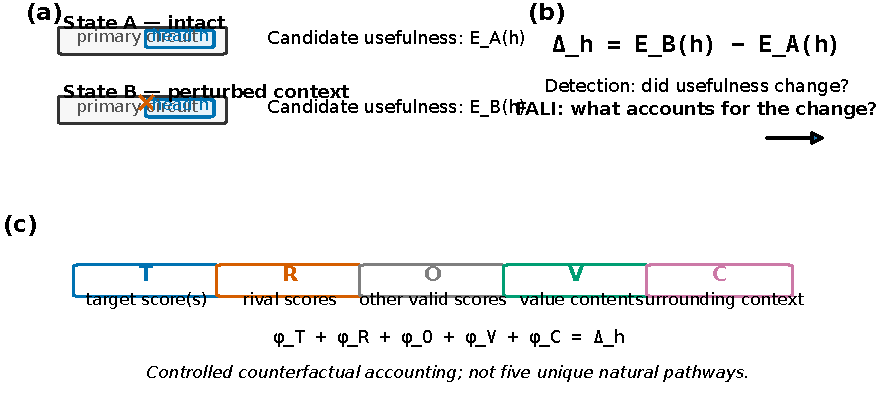
\includegraphics[width=\textwidth]{figures/Fig1.pdf}
\caption{\textbf{FALI resolves a conditional change in a selected attention head's causal usefulness.}
(a) The same candidate head $h$ is evaluated in an intact state $A$ and a prespecified perturbed state $B$.
(b) The quantity to be explained is the cross-state change $\Delta_h=E_B(h)-E_A(h)$ in output-grounded causal usefulness.
(c) FALI attributes this endpoint change under an explicit intervention game across task-target scores ($T$), rival scores ($R$), other structurally valid scores ($O$), value content ($V$), and surrounding-network context ($C$), with Owen efficiency $\phi_T+\phi_R+\phi_O+\phi_V+\phi_C=\Delta_h$.
The candidate head and task-relevant target coordinates are specified before FALI analysis.}
\label{fig:fali-overview}
\end{figure*}

